\chapter{\label{ch:4-strategy}Analytical strategy}

\section{Data}

\section{Sample selection}\label{app:imaging}


\section{Variables}\label{sub:diagnostic}

\subsection{Explanatory variable}


\subsubsection{Selection of feature set}

\begin{table}[h!]
    \centering
    \caption{Hardware --- devices used to access the Internet}
    \label{tab:hardware}
    \begin{tabular}{ll}
        \toprule
        Wave 9 (N = 6) & Wave 10 (N = 5) \\
        \midrule
        Desktop & Desktop \\
        Laptop & Laptop \\
        Tablet & Tablet \\
        Smartphone & Smartphone \\
        Other devices & Other devices \\
        Do not use any device & \\
        \bottomrule
    \end{tabular}
\end{table}


\begin{table}[h!]
    \centering
    \caption{Software --- online activities}
    \label{tab:software}
    \begin{tabular}{ll}
        \toprule
        Wave 9 (N = 16) & Wave 10 (N = 21) \\
        \midrule
        Emails & Emails \\
        Video calls & Video calls \\
        Finding information (learning) & Finding information \\
        Finding information (health) & \\
        Finances & Finances \\
        Shopping & Shopping \\
        Selling & Selling \\
        Social networking & Social networking \\
        Creating content & \\
        News & News \\
         & TV/radio \\
        Music & Music \\
        Games & Games \\
         & E-books \\
        Job application & Job application \\
        Government services & Government services \\
         & Checking travel times \\
         & Satellite navigation \\
         & Buying public transport tickets \\
         & Booking a taxi \\
         & Finding local amenities \\
         & Controlling household appliances \\
        Other online activities & \\
        No online activities & No online activities \\
        \bottomrule
    \end{tabular}
\end{table}

\subsubsection{Principal component analysis}


\begin{equation}
    \label{eq:pca_loadings}
    Z = \phi_{1}X_1 + \phi_{2}X_2 + \ldots + \phi_{p}X_p
\end{equation}


\begin{equation}
    \label{eq:pca_variance}
    \frac{1}{n} \sum_{i=1}^{n}Z_{im}^2 = \frac{1}{n} \sum_{i=1}^{n} \left( \sum_{j=1}^{p} \phi_{jm}X_{ij} \right)^2
\end{equation}


\begin{equation}
    \label{eq:pca_total_variance}
    \sum_{j=1}^{p} \frac{1}{n} \sum_{i=1}^{n}Z_{im}^2 = \sum_{j=1}^{p} \frac{1}{n} \sum_{i=1}^{n}X_{ij}^2
\end{equation}


\begin{equation}
    \label{eq:pca_algorithm}
    \textnormal{maximise}_{\phi_{11}, \ldots, \phi_{p1}} \left\{ \frac{1}{n} \sum_{i=1}^{n} \left( \sum_{j=1}^{p} \phi_{j1} X_{ij} \right)^2 \right\} \textnormal{subject to} \sum_{j=1}^{p} \phi_{j1}^2 = 1
\end{equation}

\subsection{Outcome variables}
\subsubsection{Self-rated health}

\subsubsection{Physical health}

\subsubsection{Mental health}


\begin{table}[h!]
    \centering
    \caption{Eight-item version of the CES-D scale}
    \label{tab:cesd}
    \begin{threeparttable}
        \begin{tabular}{lll}
            \toprule
            Item & Description & Positively worded \\
            \midrule
            1 & Whether felt depressed much of the time & No \\
            2 & Whether felt everything did was an effort & No \\
            3 & Whether felt sleep was restless & No \\
            4 & Whether was happy much of the time & Yes \\
            5 & Whether felt lonely much of the time & No \\
            6 & Whether enjoyed life much of the time & Yes \\
            7 & Whether felt sad much of the time & No \\
            8 & Whether could not get going much of the time & No \\
            \bottomrule
        \end{tabular}
        \begin{tablenotes}
            \footnotesize
            \item Notes: A positively worded item is one where an affirmative response indicates lower levels of depression, while a negative response indicates higher levels of depression.
        \end{tablenotes}
    \end{threeparttable}
\end{table}

\subsection{Control variables}

\begin{figure}
    \centering
    \caption{Structure of household income in IFS derived variables dataset}
    \label{fig:household_income}
    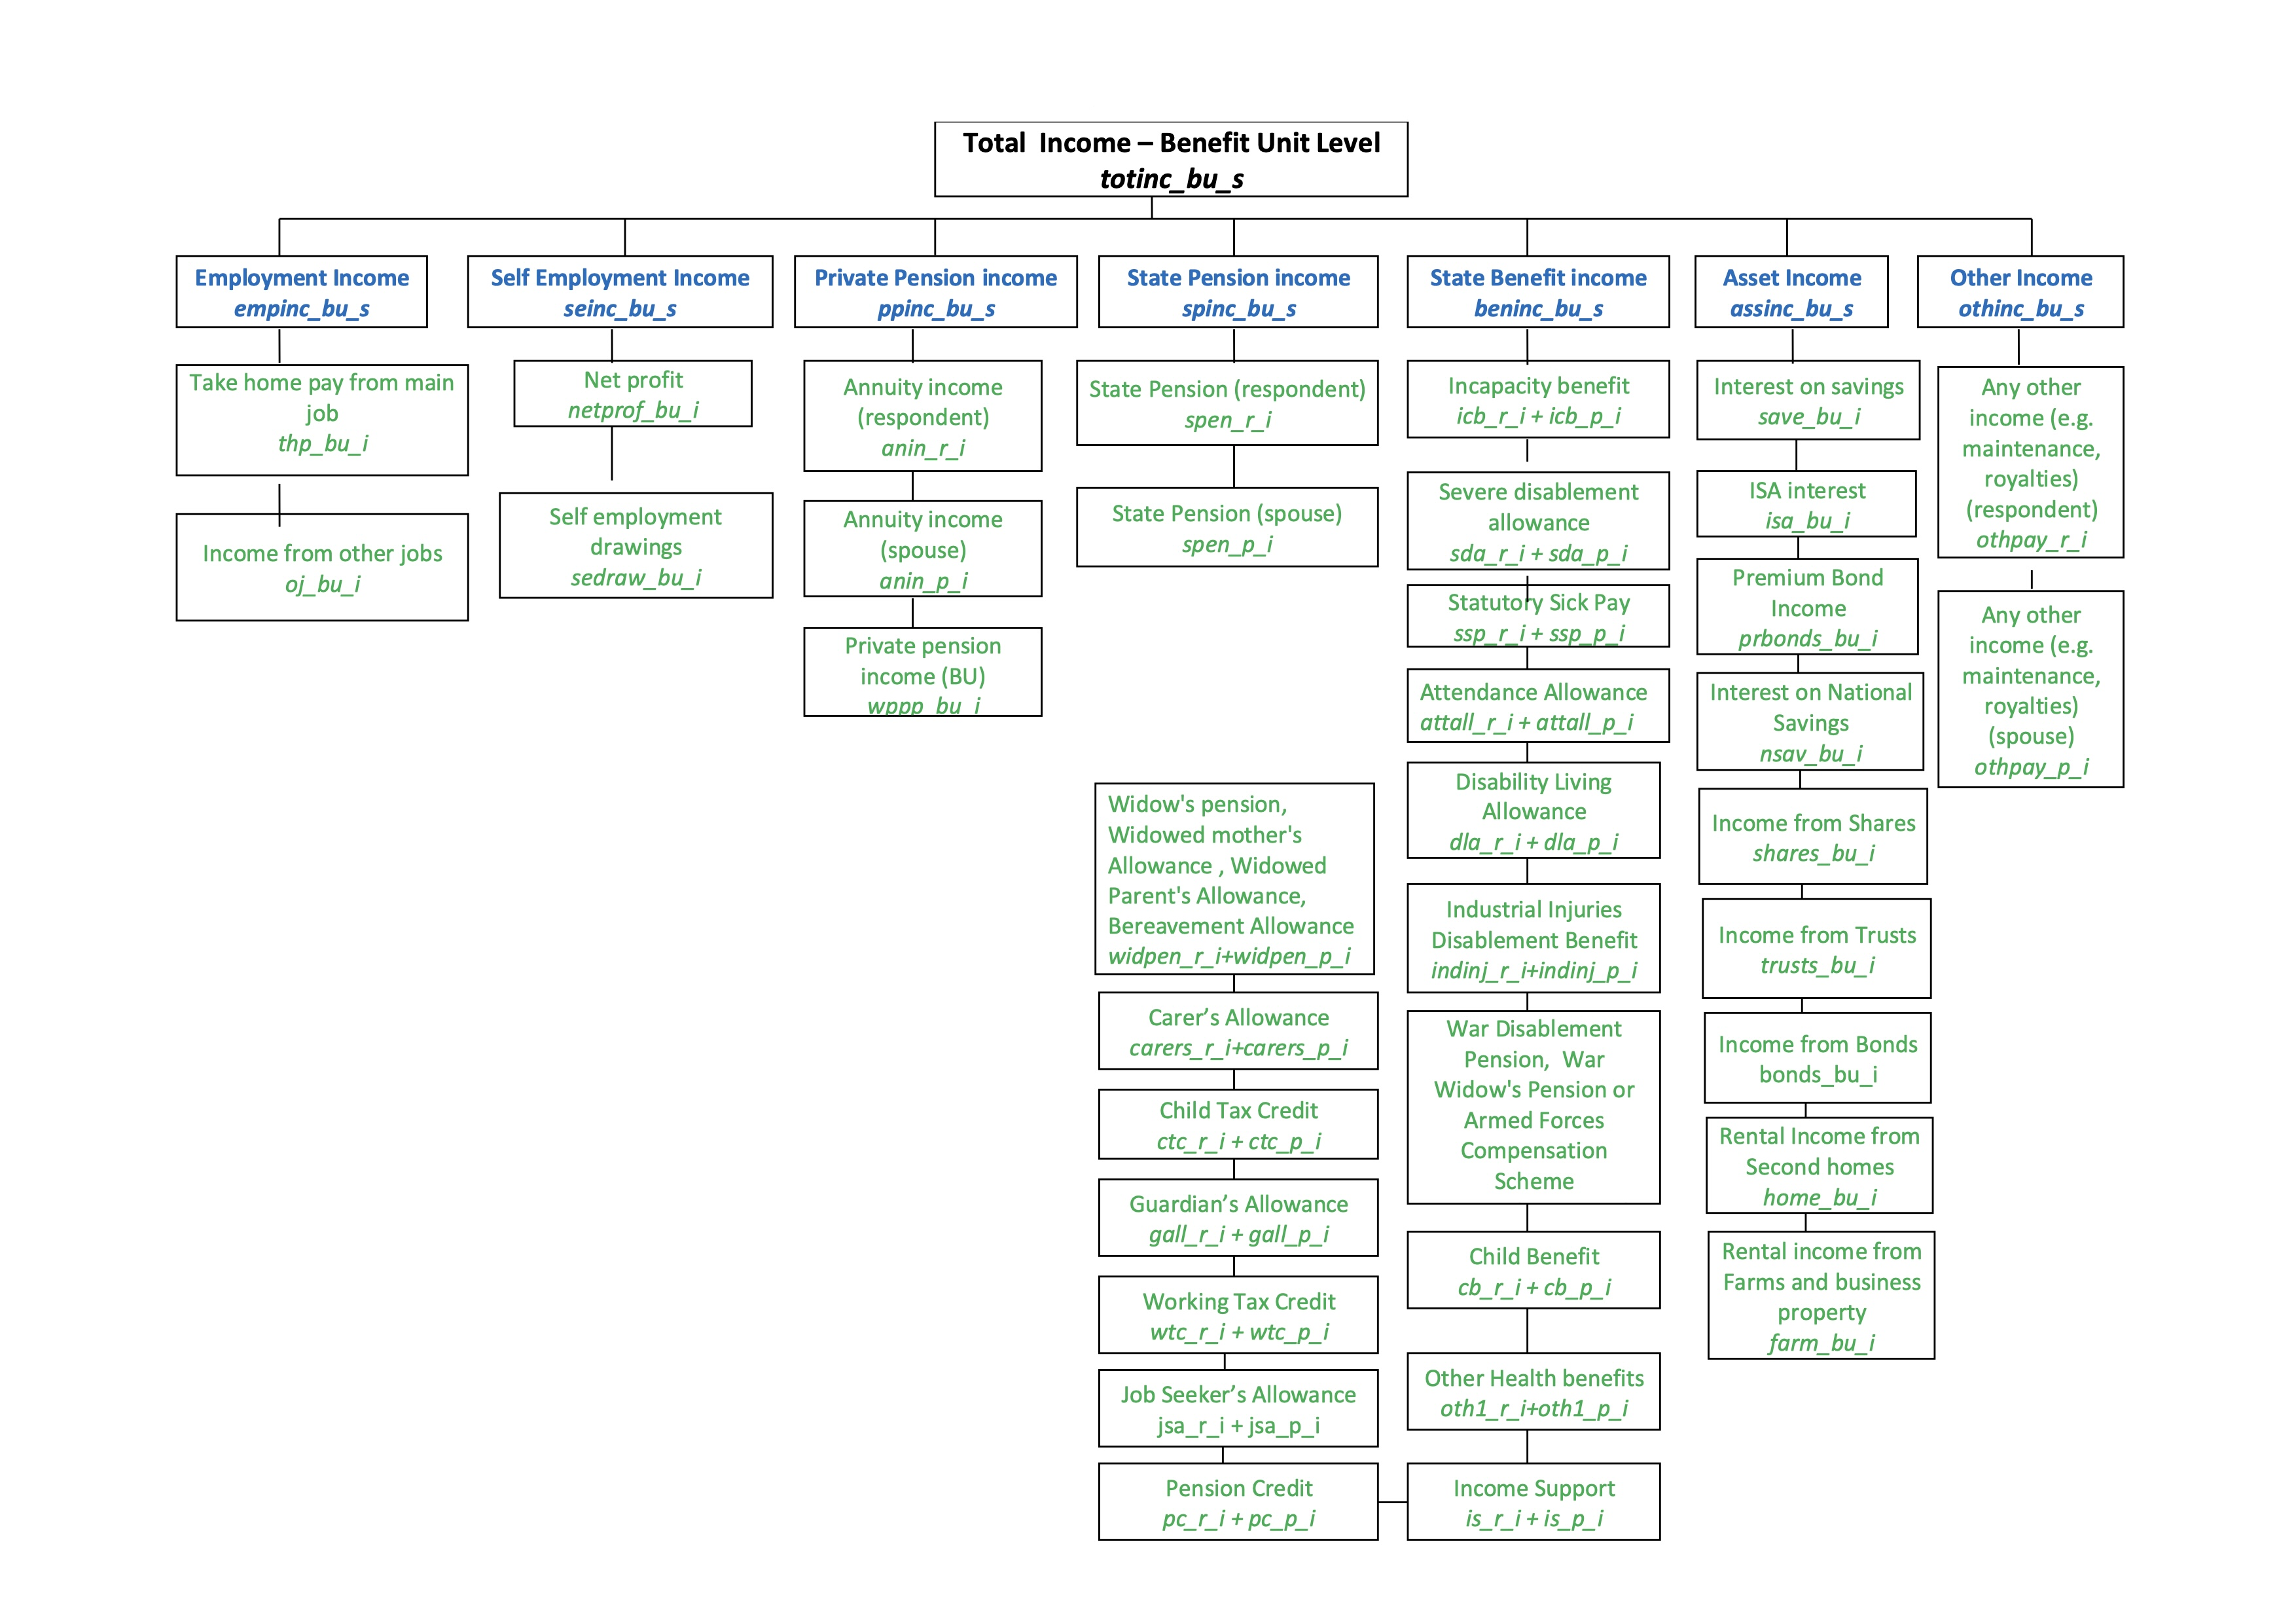
\includegraphics[width=0.8\textwidth]{figures/household_income.jpg}
\end{figure}


\begin{table}[h!]
    \centering
    \caption{Comprehension ability questions}
    \label{tab:comprehension}
    \begin{tabular}{ll}
        \toprule
        Item & Description \\
        \midrule
        1 & What is the maximum number of days you may take this medicine? \\
        2 & List three situations for which you should consult a doctor. \\
        3 & List one condition for which you might take the Medco tablet. \\
        4 & List one condition for which you should not take the Medco tablet. \\
        \bottomrule
    \end{tabular}
\end{table}